\section{Conmutación Segmentada}\label{sec:p02intro}\pagenumbering{arabic}

\subsection{Objetivo}\label{ssec:p02objetivo}

\normalsize Entender el problema de los deadlocks, y saber reproducirlos.

\subsection{Desarrollo}\label{ssec:p02desarrollo}

Se trata de crear una situación de interbloqueo (\emph{deadlock}) en diferentes topologías o en su caso analizar las circunstancias que lo impiden.

\begin{keyconceptbox}[Interbloqueo]
    También llamado bloqueo mortal (\emph{deadlock}), consiste en una dependencia de \emph{A} en \emph{B} y de \emph{B} en \emph{A} en el mismo instante de tiempo. Esto ocurre cuando, durante su recorrido, un recurso (e.g. un buffer) requerido por \emph{A} está siendo utilizado por \emph{B}. Al mismo tiempo, durante su recorrido, \emph{B} requiere del uso de un recurso que está siendo utilizado por \emph{A}. De esta manera, ninguno de los dos podrá avanzar, ya que dichos recursos no podrán ser liberados nunca.

    \vspace{10pt}

    \centering 	\fbox{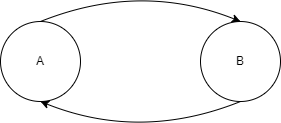
\includegraphics[width=0.5\linewidth]{figs/diagrama-interbloqueo.drawio.png}} \label{fig:diagrama-interbloqueo}
    
\end{keyconceptbox}

\begin{itemize}
    \item[\textbf{a)}] \textbf{Un caso muy sencillo se puede obtener en una red de interconexión con topología toro 2D, considerando canales unidireccionales.}

    Para obtener un interbloqueo en una dimensión, es conveniente (y para dimensiones de cuatro nodos, necesario) que los paquetes recorran el camino más largo posible. De esta manera, será más probable que ambos paquetes se encuentren en sus caminos. Asimismo, es necesario que ambos paquetes salgan de nodos situados a la mayor distancia posible entre ellos ya que, de lo contrario, con cuatro nodos se rompería cualquier ciclo posible. La Figura \ref{fig:interbloqueo-simured} muestra una situación de interbloqueo en la que el paquete A sale del nodo 0 al 1, y el paquete B del nodo 2 al 3. Véase que si hubiéramos lanzado el paquete B desde el nodo 1 al 2, se rompería el ciclo de dependencia, ya que el paquete A podría alcanzar el nodo 1 sin problemas.

    \begin{figure}[h] % Adjust the width as needed
      \centering
      \fbox{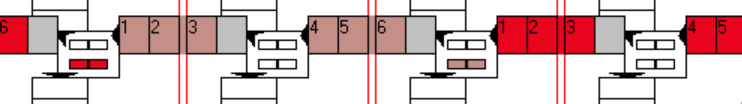
\includegraphics[width=0.9\textwidth]{figs/interbloqueo-zoom.png}} % Replace with your image filename
      \caption{Interbloqueo en Simured.}
      \label{fig:interbloqueo-simured}
    \end{figure}

    \item[\textbf{b)}] \textbf{Plantear casos más complejos que intervengan nodos de dos dimensiones distintas, utilizando la topología que consideréis oportuna y aplicando canales bidireccionales o unidireccionales. En su caso si no se consigue el bloqueo analizar las circunstancias que lo impiden.}\par
    \textbf{En todos los casos, se utilizará el simulador \emph{SimuRed}, descrito en el apéndice A.}

    En este caso el interbloqueo se tiene que dar de tal manera que todos los paquetes tengan que utilizar las dos dimensiones en su recorrido. Para ello, y en primer lugar, hay que utilizar un algoritmo de encaminamiento totalmente adaptativo, ya que de lo contrario se rompería cualquier ciclo. En segundo lugar, los canales tienen que ser bidireccionales. En tercer lugar, en este caso será necesario lanzar cuatro paquetes. Por último, la longitud del paquete debería ser mayor que el doble de la longitud de las colas. En este caso, para generar el interbloqueo, hay que lanzar los paquetes en cruz. El Listing \ref{lst:traza2b} muestra un ejemplo de traza que enviaría los paquetes en cruz. 

    \begin{mycode}[style=mycodestyle, caption={Traza para provocar un interbloqueo en dos dimensiones.}, label=lst:traza2b]
0 9 6
0 6 9
0 10 5
0 5 10
    \end{mycode}

    Al utilizar un algoritmo de encaminamiento determinista, es posible que no se produzca un interbloqueo a la primera. Por eso, es probable que se tengan que realizar varias ejecuciones con la misma traza hasta que aparezca. La Figura \ref{fig:interbloqueo-2d} muestra un posible interbloqueo en dos dimensiones usando Simured.

    \begin{figure}[h] % Adjust the width as needed
      \centering
      \fbox{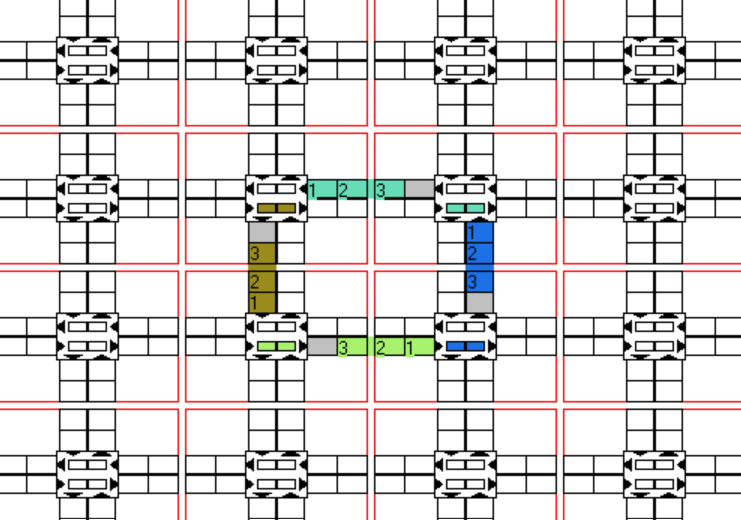
\includegraphics[width=0.7\textwidth]{figs/interbloqueo-2d.png}} % Replace with your image filename
      \caption{Interbloqueo en dos dimensiones.}
      \label{fig:interbloqueo-2d}
    \end{figure}

\end{itemize}